\documentclass{article}
\usepackage{microtype}
\usepackage{graphicx}
\usepackage{booktabs}
\usepackage{hyperref}
\hypersetup{hypertexnames=false}
\newcommand{\theHalgorithm}{\arabic{algorithm}}
\usepackage[accepted]{icml2025}
\usepackage{amsmath,amssymb}
\makeatletter
\renewcommand{\Notice@String}{Independent experimental report, October 2026.
Official ICML 2025 format; not a conference submission or publication.}
\gdef\icmlcorrespondingauthor@text{reproduction instructions in the accompanying README}
\makeatother
\icmltitlerunning{Simple Predictions of Small-Graph Cover Times}
\begin{document}
\twocolumn[
\icmltitle{Simple Predictions of Uniform-Start Random-Walk Cover Times
on Small Graphs: Accuracy and Family Dependence}
\begin{icmlauthorlist}
\icmlauthor{Autonomous Research Agent}{report}
\end{icmlauthorlist}
\icmlaffiliation{report}{Independent reproducible experiment}
\icmlkeywords{random walks, cover time, small graphs, Monte Carlo}
\vskip 0.3in
]
\printAffiliationsAndNotice{}

\begin{abstract}
Can a few inexpensive graph statistics predict random-walk cover times more
closely than a general upper bound? We generate 133 connected graphs with
8--30 vertices from ten families and estimate their uniform-start mean cover
times with 4,000 independent walks each. A fixed log-linear ridge model using
vertex count, edge count, maximum degree, and diameter achieves a
family-balanced test mean absolute percentage error of 20.1\%, with a
Monte Carlo 95\% interval of [19.8, 20.5]\%, compared with 75.9\% for a fitted
size-only model. Accuracy depends strongly on family: errors are about 5\%
on stars but 50--55\% on grids and dense random graphs. Leaving an entire
family out of training raises overall error to 31.3\%. These results support
a useful empirical approximation on this graph collection, without a
uniform accuracy guarantee over small connected graphs.
\end{abstract}

\section{Introduction}
For a simple random walk on a finite connected undirected graph, the time to
visit all vertices varies substantially with topology. General bounds,
including the classical edge-based bound associated with random-walk
traversal \citep{aleliunas1979}, give guarantees but need not approximate
individual instances. Tight extremal bounds \citep{feige1995} address a
different objective from typical-instance prediction. The survey of
\citet{lovasz1993} provides background on random walks on graphs.

We test four basic statistics on held-out sizes and unseen families,
with saved raw trajectories and propagated simulation uncertainty.
Under the task's access restriction, no research literature or discussing
pages were retrieved; we make no novelty claim. The supplied references
serve as background; all numerical evidence was generated here.

\section{Method}
\paragraph{Target and estimator.}
Let $G=(V,E)$, $n=|V|$, $m=|E|$, and let $X_0$ be uniform on $V$.
At each step, the walk chooses a neighbor uniformly. We study
\begin{equation}
 C_U(G)=\mathbb{E}\big[\min\{t:\{X_0,\ldots,X_t\}=V\}\big].
\end{equation}
Thus the initial vertex is visited at time zero. This target averages over
starting vertices; it is not the frequently used worst-start quantity
$\max_v\mathbb{E}_v[T]$. For each graph we simulate $R=4000$ independent
walks, independently resampling the initial vertex each time, with no
trajectory cutoff. The label $\widehat C_U$ is their sample mean; its standard
error is the sample standard deviation divided by $\sqrt R$. We save every
integer cover time and report a Student-$t$ approximate 95\% interval for
each graph mean.

\paragraph{Predictors.}
Our four features are $x=(\log n,\log m,\log\Delta,\log D)$, where
$\Delta$ is maximum degree and $D$ is diameter. Average degree $2m/n$ adds
no independent information. Breadth-first searches compute $D$ in
$O(n(n+m))$ time, negligible here. Feature means and standard deviations
are computed on training graphs only. Writing standardized features as $z$,
we fit $\log\widehat C_U$ by minimizing
\begin{equation}
 \sum_{g\in\mathcal T}w_g
 (\log\widehat C_U(g)-b-\beta^\top z_g)^2
 +0.01\|\beta\|_2^2,
\end{equation}
where weights sum to one, every family has equal total weight, and graphs
within each family have equal weight. The intercept is unpenalized.
Predictions are $\exp(b+\beta^\top z)$, with no correction or clipping.
The feature set, penalty, and splits were fixed before inspecting scores;
we perform no hyperparameter search.

We compare with the same fitted procedure using only $\log n$, and with
$B(G)=2m(n-1)$, a valid general upper bound on worst-start cover time and
hence on $C_U$. A bound is a deliberately conservative reference, not a
competitive learned predictor. We do not use an asymptotic extremal formula
as a finite-$n$ guarantee.

\paragraph{Evaluation and uncertainty.}
For a set of graphs, define MAPE as the family-balanced average of
$100|\widehat C_{\rm pred}/\widehat C_U-1|$. We also report the multiplicative
error factor $\exp(\operatorname{avg}|\log(\widehat C_{\rm pred}/\widehat C_U)|)$
using the same weights. A factor of one is perfect.

To propagate Monte Carlo noise through both fitting and evaluation, we
partition each graph's 4,000 independent times into 40 blocks of 100.
In each of 500 bootstrap repetitions we independently resample the 40
block means for every graph, reconstruct its mean, refit every model,
and recompute scores. Brackets in the tables are the 2.5th and 97.5th
percentiles. These are approximate Monte Carlo intervals conditional on
the fixed graph collection, not uncertainty over unseen graphs, a
prediction interval, or a guarantee of model accuracy. Graphs, rather
than individual trajectories, are the units of prediction.

\section{Experiments}
\paragraph{Graph collection and splits.}
We use $n\in\{8,12,16,20,24,28,30\}$. Seven deterministic families have one
graph per size: path, cycle, star, clique, grid, lollipop, and barbell.
The grid comprises vertices $0,\ldots,n-1$ arranged in rows of width
$\lfloor\sqrt n\rfloor$, with horizontal and vertical lattice edges;
the final row may be incomplete. The lollipop has a clique of
$\lceil n/2\rceil$ vertices attached to a path on the remaining vertices.
The barbell has two cliques of size $\lfloor n/3\rfloor$, joined through
a path with $n-2\lfloor n/3\rfloor$ internal vertices.
Three stochastic families have four independent graphs per size:
$G(n,3/(n-1))$, $G(n,0.35)$, and uniform labeled trees generated from
uniform Pr\"ufer sequences. ER graphs are rejection-sampled until connected.
The sparse/dense names refer to the parameter rules, not to an ordering
of realized densities at every size.

Training sizes are $\{8,12,20,28\}$ (76 graphs); testing sizes are
$\{16,24,30\}$ (57 graphs), including a small extrapolation to 30.
No deterministic graph is duplicated across splits. A separate
leave-one-family-out (LOFO) evaluation fits on all sizes of nine families
and tests all sizes of the remaining family, repeated ten times.
LOFO and held-out-size results therefore answer different questions.
The global seed is 20261027; graph-specific seeds and edge lists are stored.
The complete CPU experiment takes under one minute, including compilation,
simulation, fitting, and 500 bootstraps.

\paragraph{Simulation checks.}
For every sampled size we compare against three analytic uniform-start
expectations. With $L=n-1$ and $H_L=\sum_{k=1}^L1/k$, these are
$L^2+L(L-1)/6$ for a path, $LH_L$ for a clique, and
$2LH_L-(2n-1)/n$ for a star. For a path, first hit either endpoint
(mean $i(L-i)$ from position $i$) and then traverse to the opposite endpoint
(mean $L^2$); averaging gives the formula. The clique and star expressions
follow from collecting previously unseen vertices or leaves.
Across these 21 checks, the largest absolute standardized discrepancy
is 2.66 standard errors; 19 of 21 approximate 95\% intervals contain
the analytic value. This is a numerical check rather than proof of
correctness. Across all 133 graphs, the median relative 95\% interval
half-width is 1.65\%, with maximum 3.76\%.

\begin{table}[t]
\caption{Family-balanced errors. Brackets: 95\% Monte Carlo intervals
for MAPE. First three rows use held-out sizes; LOFO rows use separate
family folds over all sizes. The factor is the exponentiated mean absolute
log error.}
\label{tab:overall}
\centering\small
\begin{tabular}{lrr}
\toprule
Predictor & MAPE (\%) & Factor\\
\midrule
Upper bound & 2151.1 [2142.5, 2161.7] & 7.26 \\
Size-only & 75.9 [75.4, 76.4] & 1.96 \\
Four statistics & 20.1 [19.8, 20.5] & 1.20 \\
LOFO size-only & 75.4 [75.1, 75.8] & 1.94 \\
LOFO four stats. & 31.3 [31.1, 31.6] & 1.41 \\
\bottomrule
\end{tabular}

\end{table}

\begin{figure*}[t]
\centering
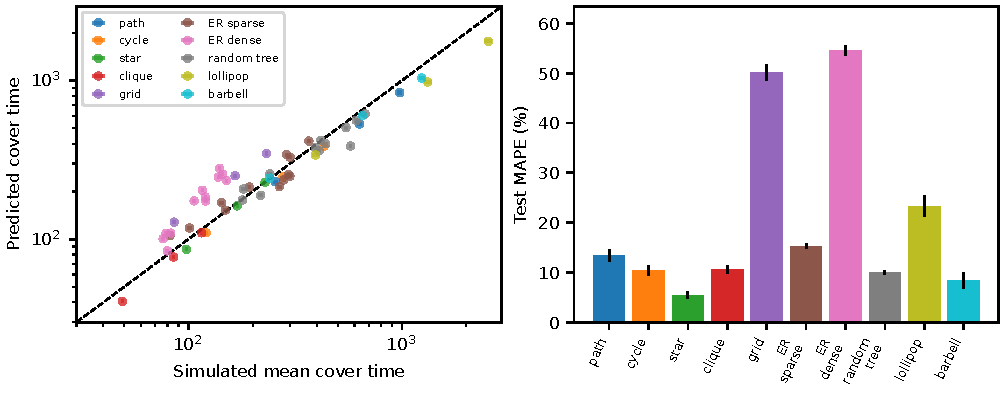
\includegraphics[width=\textwidth]{figures/results.pdf}
\caption{Held-out-size predictions of the four-statistic model.
Left: predicted versus simulated cover time, with horizontal 95\%
Monte Carlo error bars and a dashed equality line. Right: family-wise MAPE;
black intervals propagate Monte Carlo uncertainty through refitting.
These intervals do not measure variability over a population of graphs.}
\label{fig:results}
\end{figure*}

\paragraph{Overall predictive accuracy.}
Table~\ref{tab:overall} shows a reduction from 75.9\% to 20.1\% MAPE when
moving from size alone to four statistics; the multiplicative error factor
falls from 1.96 to 1.20. The general upper bound is much looser, with
2151\% MAPE. That comparison alone would give weak evidence of usefulness;
the fitted size baseline provides the more informative comparison.
The fitted four-statistic rule, rounded for readability, is
\begin{equation}
 \widehat C_{\rm pred}\simeq
 0.602\,n^{0.786}m^{0.031}\Delta^{0.696}D^{1.182}.
\end{equation}
Full-precision standardized coefficients are saved for reuse.
Because features are correlated and the model is regularized, these
exponents should not be interpreted as causal scaling laws.

\begin{table}[t]
\caption{MAPE (\%) by graph family for the four-statistic model.
Size-test brackets denote Monte Carlo 95\% intervals.
LOFO tests the entire omitted family over all seven sizes.}
\label{tab:families}
\centering\small
\begin{tabular}{lrr}
\toprule
Family & Size test & LOFO\\
\midrule
path & 13.3 [12.1, 14.6] & 14.8 \\
cycle & 10.4 [9.4, 11.4] & 16.4 \\
star & 5.3 [4.8, 6.1] & 42.2 \\
clique & 10.5 [9.8, 11.3] & 58.9 \\
grid & 50.1 [48.6, 51.8] & 56.9 \\
ER sparse & 15.2 [14.7, 15.8] & 16.7 \\
ER dense & 54.6 [53.6, 55.6] & 58.0 \\
random tree & 10.0 [9.5, 10.4] & 11.1 \\
lollipop & 23.3 [21.2, 25.5] & 31.9 \\
barbell & 8.3 [6.7, 9.9] & 6.3 \\
\bottomrule
\end{tabular}

\end{table}

\paragraph{Family dependence and transfer.}
The family breakdown (Table~\ref{tab:families}, Figure~\ref{fig:results})
shows that stars, random trees, and barbells have approximately 5--10\%
held-out-size error. Paths, cycles, cliques, and sparse ER graphs have
10--15\% error, while lollipops have 23\% error. The largest errors occur
on grids (50\%) and dense ER graphs (55\%), both systematically
overpredicted on these test graphs. Lollipops are systematically
underpredicted. Bottlenecks are therefore not the only difficult case.
Nor is adding statistics uniformly better: the size-only baseline's
cycle error is 5.6\%, versus 10.4\% for four statistics.

LOFO MAPE increases to 31.3\% [31.1, 31.6], still below its size-only
counterpart (75.4\%), but stars and cliques now have 42\% and 59\% error.
Thus low error within a represented family does not imply successful
transfer to a previously unrepresented family. In contrast, barbell and
random-tree LOFO errors remain about 6\% and 11\%.

\section{Discussion and Limitations}
Four elementary statistics provide a substantially better approximation
than the chosen general bound and a fitted size baseline on this collection.
Nevertheless, the family-wise errors are far larger than the simulation
uncertainty, indicating model mismatch rather than insufficient walks.
The large grid and dense-ER errors are consistent with the limited
flexibility of a single multiplicative rule. Diameter and maximum degree
do not encode all spatial organization or bottleneck structure. Our
experiment does not isolate which omitted property causes each error.

This is a connectivity smoke test, not an exhaustive benchmark: it includes
only seven sizes from 8 upward, a few instances per random family, and
specific lollipop/barbell proportions. In particular, nothing here
establishes a guarantee for every graph with at most 30 vertices, for
$n<8$, for different starting distributions, or for worst-start cover
time. Family balancing is a deliberate evaluation choice, not a natural
distribution on all connected graphs. Small Monte Carlo intervals should
not be mistaken for confidence in out-of-distribution predictions.

The predictor is a rough estimate for represented families and sizes;
applications should validate on their own graph class. Predictions are
not certified upper bounds. More flexible models remain untested.
Code, raw outcomes, seeds, and compilation instructions accompany this report.

\bibliography{references}
\bibliographystyle{icml2025}
\end{document}
